\chapter{Resultados obtenidos en los experimentos}

El presente capítulo tiene como objetivo exponer los resultados obtenidos en las simulaciones y ciertas consideraciones descubiertas durante la implantación de los algoritmos. Para todo ello se han empleado funciones y \emph{scripts} desarrollados con \emph{MATLAB}.\par

La estructuración de los resultados se ha efectuado de tal manera que en primer lugar se analizará la estimación del observador del estado del sistema a lo largo del tiempo ante distintas situaciones, y posteriormente se mostrará el comportamiento del estimador de la fuerza externa aplicada al elemento terminal. \par 

Es preciso destacar en primer lugar, ciertos aspectos que se han descubierto a lo largo de la realización de los ensayos y que es indispensable mencionar. \par 

\newpage
\section{Aspectos a destacar de las simulaciones}
\label{sec:dificultades}

Durante la realización de las simulaciones del sistema, se han descubierto ciertos comportamientos de los \emph{plugins} desarrollados, más concretamente del sensor fuerza par codificado en \emph{C++}, los cuales proporcionan valores anómalos en los datos, por lo que se han considerado como errores a corregir por parte de los desarrolladores del motor físico de \emph{Gazebo} o fallos en el código desarrollado para la realización de los \emph{plugins}. \par 

Las distintas situaciones en las que se han encontrado sucesos extraños serán descritas y acompañadas por gráficas obtenidas con \emph{MATLAB}, las cuales simplemente representan en el eje de ordenadas el valor en $N$ o $Nm$ de las fuerzas y momentos, respectivamente, medidas por el sensor, y en el eje de abscisas el tiempo en $s$ o $ms$. \par 

\noindent
Dichos comportamientos se muestran a continuación:

\begin{itemize}
\item Tras lanzar la simulación, estando estático el manipulador, el sensor fuerza par mide una fuerza en dirección del eje x (paralelo al plano horizontal y perpendicular al eje de rotación del último grado de libertad) de alrededor de 1N en ciertas ocasiones (color azul en figura \ref{fig:errorFTsensor1}), y alrededor de 10N en otras, debiendo ser esta componente nula.

\begin{figure}[h!]
\centering
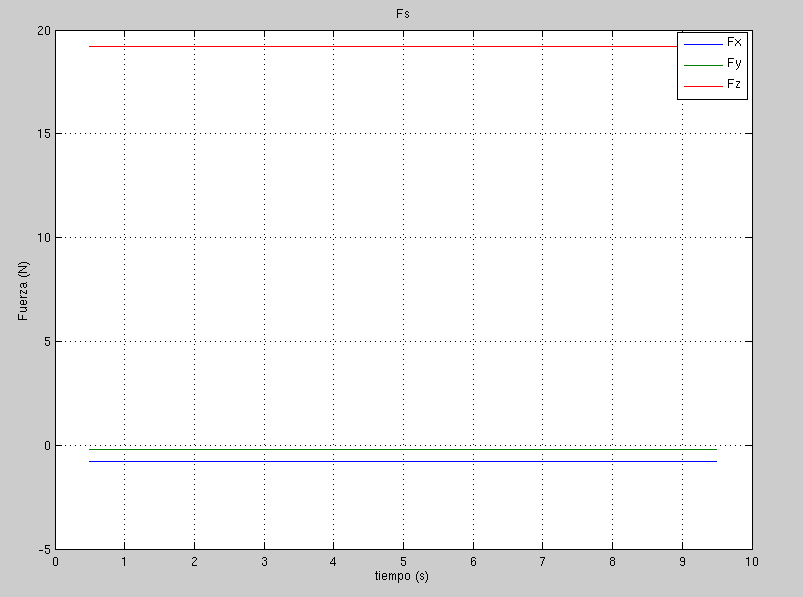
\includegraphics[scale=0.6]{Figuras/FTerror1}
\caption{Medida del sensor fuerza par simulado a 500 Hz sin movimiento ni fuerza externa. Se puede observar una fuerza residual de 1N de amplitud en dirección del eje $x$ (color azul).}
\label{fig:errorFTsensor1}
\end{figure}

\item Esta fuerza en dirección del eje x aparece únicamente en la posición inicial del manipulador. Si se efectúa un pequeño desplazamiento, en este caso de 0.1 rad alrededor del primer grado de libertad, \acrshort{gdl}, (eje perpendicular al plano horizontal), esta componente desaparece, tal y como se aprecia en la figura \ref{fig:errorFTsensor2}.

\begin{figure}[h!]
\centering
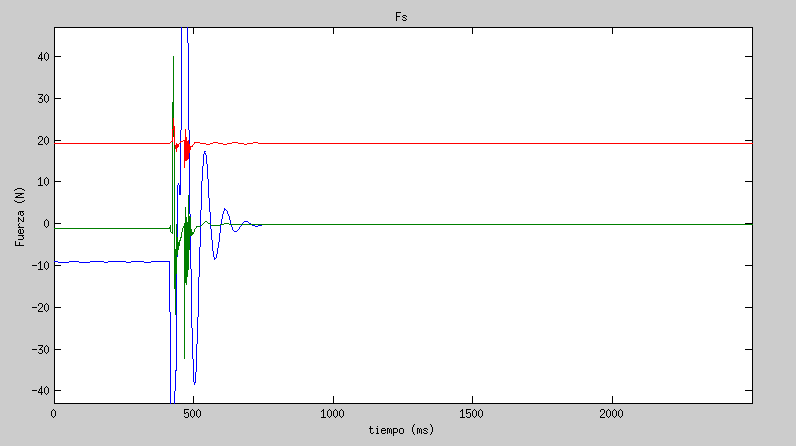
\includegraphics[scale=0.5]{Figuras/FTerror2}
\caption{Medida del sensor fuerza par simulado a 500Hz al efectuar un giro de 0.1 rad alrededor del primer GDL.}
\label{fig:errorFTsensor2}
\end{figure}

Pueden apreciarse también las oscilaciones que aparecen tras el paso de ciertos milisegundos una vez parado el manipulador. Este comportamiento podría ser resultado del controlador empleado, pero dichas oscilaciones no aparecen reflejadas en el sensor inercial, lo que produce una estimación errónea de las fuerzas externas. \par 

\item Si en cambio, en vez de efectuar un movimiento se aplica una fuerza externa durante cierto tiempo, y se deja de aplicar al cabo de ciertos segundos, se obtiene la gráfica mostrada en la figura \ref{fig:errorFTsensor3}. Se puede apreciar que la fuerza medida a lo largo del eje x es de 10N, la aplicada al extremo, por lo que esta fuerza analizada sólo aparece en reposo. \par 

Por otro lado, se observa que al cabo de ciertos milisegundos de dejar de aplicar la fuerza externa, la fuerza de 1N vuelve a aparecer. La única manera de hacerla desaparecer es efectuando un pequeño movimiento. \par 

\begin{figure}[h!]
\centering
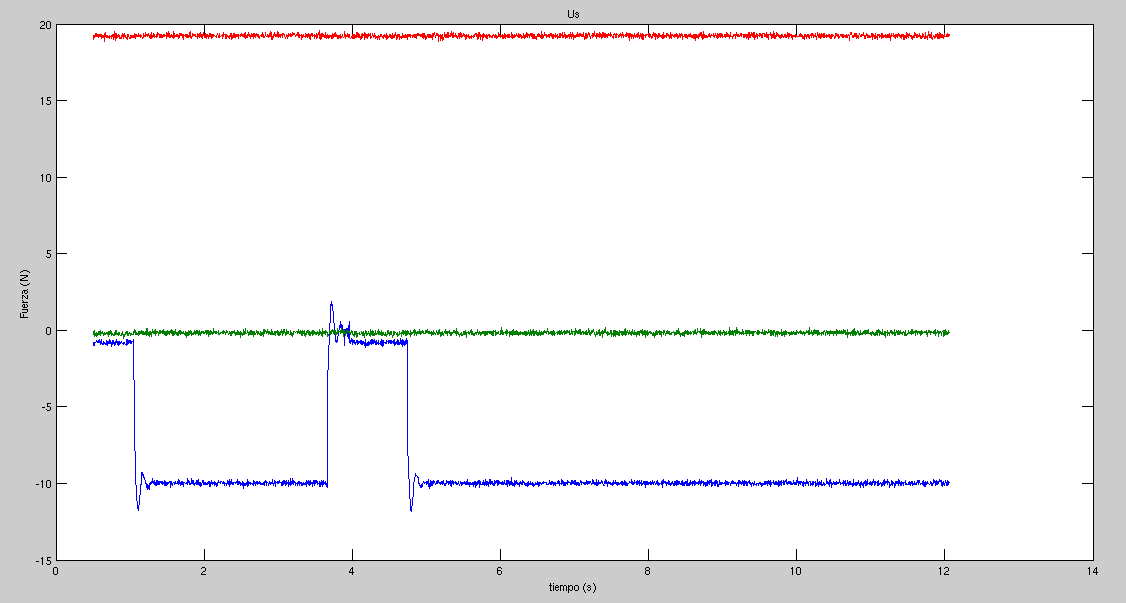
\includegraphics[scale=0.5]{Figuras/FTerror3}
\caption{Medida del sensor fuerza par simulado a 250Hz al aplicar una fuerza de manera intermitente y sin movimiento.}
\label{fig:errorFTsensor3}
\end{figure}

\item Al realizar cualquier movimiento el manipulador, el sensor fuerza par muestra ciertos 'picos' que no se encuentran reflejados en las medidas de los acelerómetros, como se muestra en la figura \ref{fig:errorFTsensor4}, la cual muestra dos gráficas obtenidas durante la misma simulación a 1KHz. Ambas deberían mostrar respuestas proporcionales, para cumplir las leyes de Newton, puesto que no se ha ejercido ninguna fuerza externa. \par 

\begin{figure}[h!]
\centering
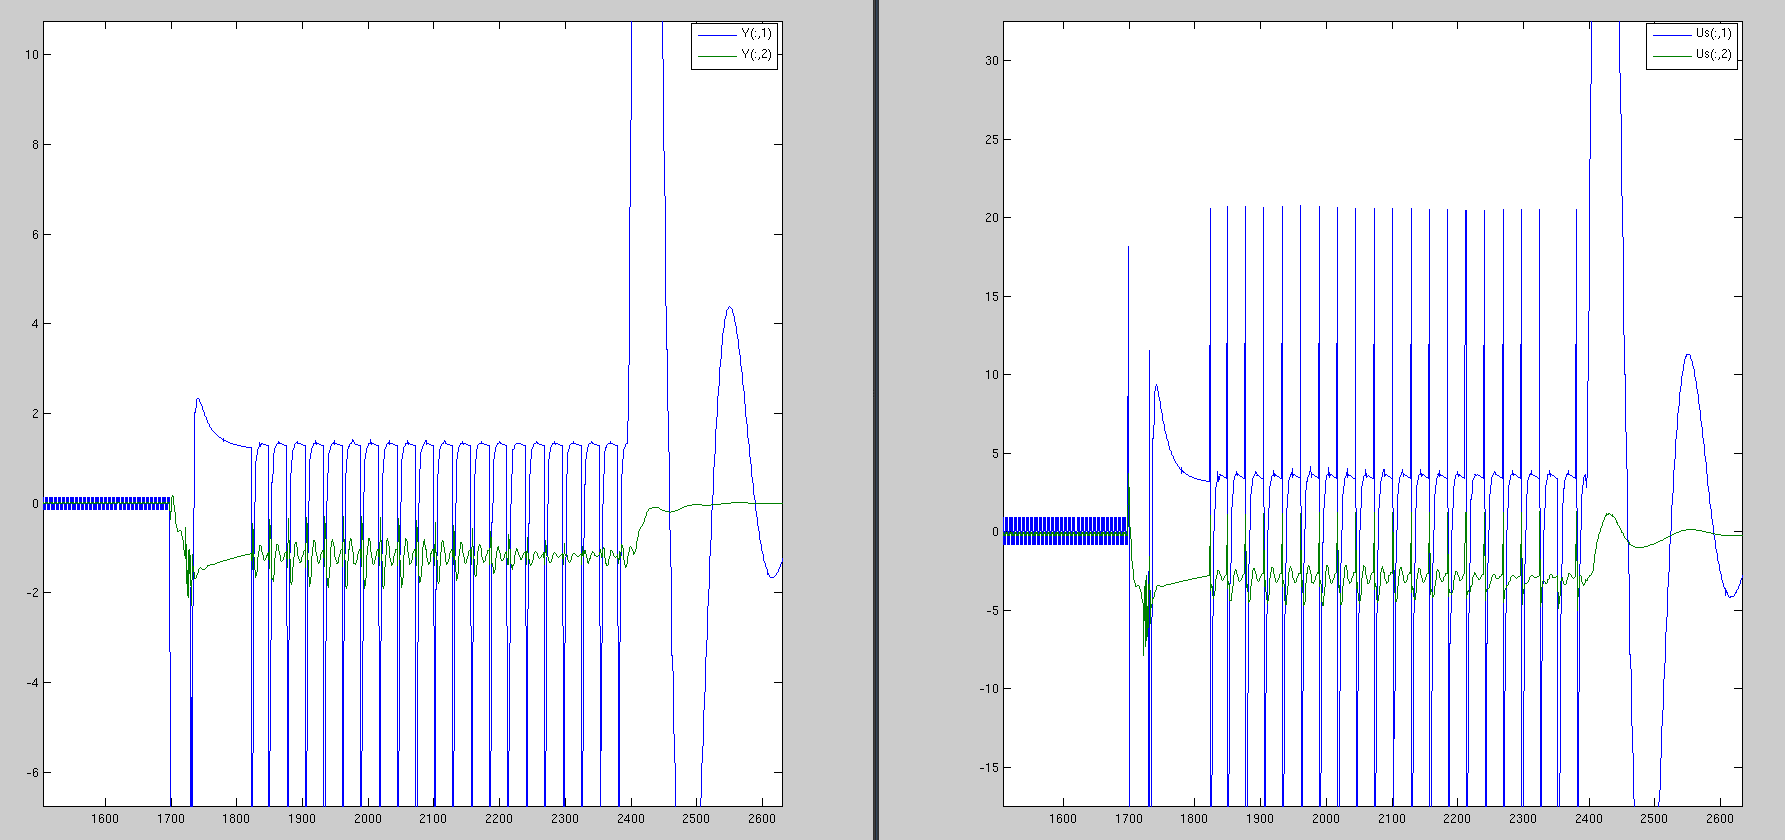
\includegraphics[scale=0.325]{Figuras/FTerror4}
\caption{A la izquierda: aceleración medida por la IMU. A la derecha: fuerza medida por el sensor fuerza par.}
\label{fig:errorFTsensor4}
\end{figure}

Se ha podido apreciar durante diversas simulaciones, que la magnitud de estos picos en la fuerza se agranda a medida que se aumenta la frecuencia de adquisición de datos del sensor, por lo que se ha determinado en los distintos ensayos una frecuencia de 500 Hz. \par 

\item Al emplear frecuencias de adquisición de datos de 1 kHz, la ideal para implementar el algoritmo en tiempo real, se obtienen medidas en los sensores que muestran elevadas oscilaciones, como se muestra en la figura \ref{fig:errorFTsensor5} para el sensor fuerza par, en la cual se ha especificado ruido nulo en los sensores. \par 

\begin{figure}[h!]
\centering
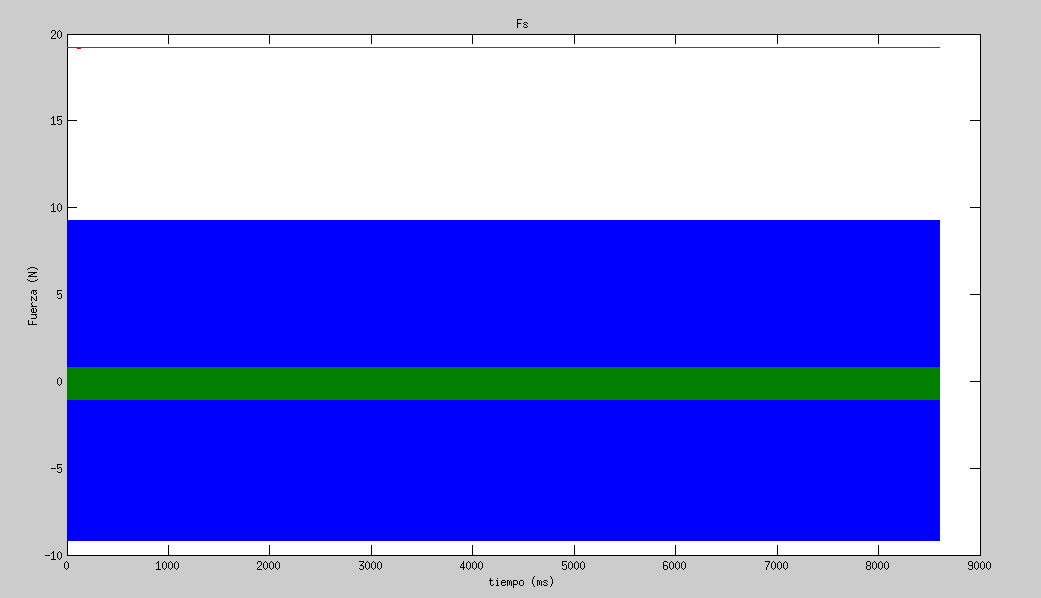
\includegraphics[scale=0.35]{Figuras/FTerror5}
\caption{Fuerza medida por el sensor fuerza par simulado, a 1kHz, sin movimiento ni fuerza externa.}
\label{fig:errorFTsensor5}
\end{figure}

El principal problema surge al calcular numéricamente la derivada de la velocidad angular para obtener una estimación de la aceleración angular, necesaria para poder implementar el algoritmo del observador, lo cual produce una amplificación de las oscilaciones, obteniéndose valores ilógicos de aceleraciones. Por esta razón y por la mencionada en el punto anterior, la frecuencia empleada es de 500 Hz. \par 

\item Al ejercer una fuerza en dirección del eje x o y (en un eje exclusivamente), se aprecia la aparición de una fuerza en el eje restante de un orden de magnitud inferior al de la fuerza externa especificada (figura \ref{fig:errorFTsensor6}). \par 

\begin{figure}[h!]
\centering
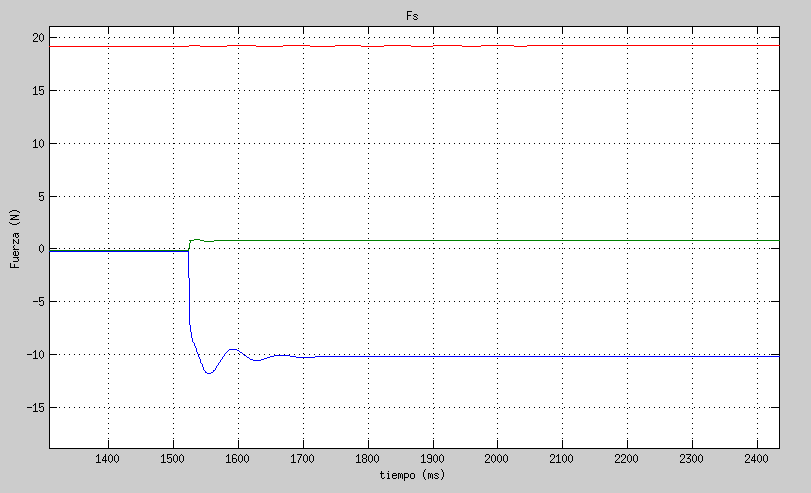
\includegraphics[scale=0.45]{Figuras/FTerror6}
\caption{Fuerza medida por el sensor fuerza par simulado, a 0.5kHz, aplicando 10N en el eje $x$.}
\label{fig:errorFTsensor6}
\end{figure}

Se puede apreciar que la fuerza medida no puede ser debida a una rotación del sistema de referencia en el que se aplica la fuerza, puesto que la fuerza total resultante presenta un módulo mayor que el de la fuerza especificada a aplicar, por lo que la causa debe ser distinta. \par  

En el caso de que se ejerza una fuerza con componentes en ambos ejes $x$ e $y$, la amplitud de la fuerza medida por el sensor no coincide con la aplicada, como se muestra en la figura \ref{fig:errorFTsensor7}, en la cual se ha ejercido una fuerza de 10N en sentido positivo del eje $x$ y otra idéntica en sentido positivo del eje $y$. \par 

\begin{figure}[h!]
\centering
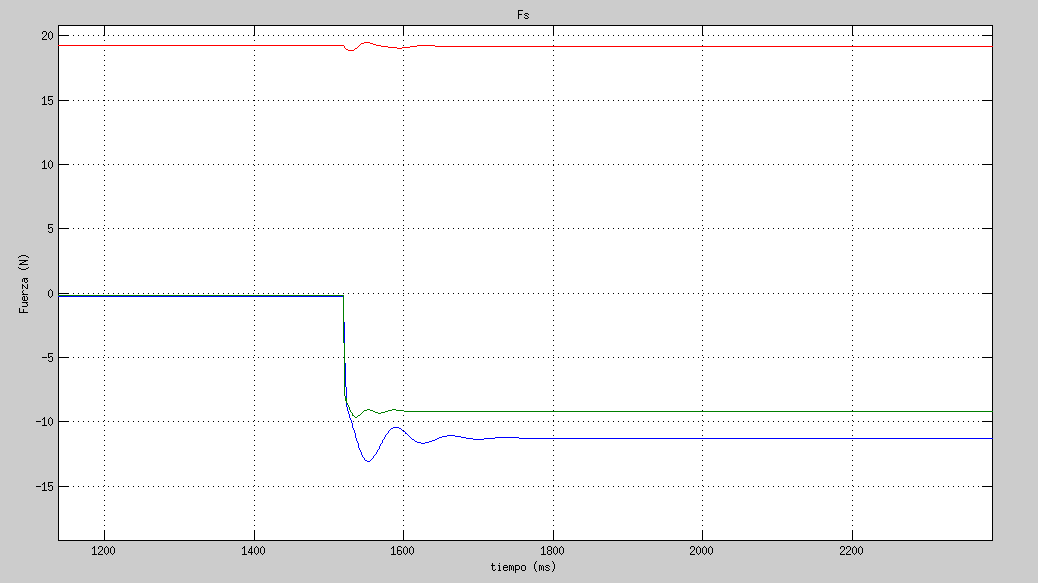
\includegraphics[scale=0.4]{Figuras/FTerror7}
\caption{Fuerza medida por el sensor fuerza par simulado, a 0.5kHz, aplicando 10N en el eje $x$ y 10N en $y$.}
\label{fig:errorFTsensor7}
\end{figure}

Puede apreciarse de nuevo en la figura \ref{fig:errorFTsensor7} que el módulo de la fuerza resultante medida por el sensor es superior al de la fuerza especificada. Esta situación se compensará ejerciendo una fuerza 10 veces inferior en el eje $y$ a la aplicada en el eje $x$, de esta manera, por ejemplo, si se ejercen 10 N en sentido positivo del eje $x$ y 1 N en sentido positivo del eje $y$, el sensor fuerza par únicamente mide una fuerza de 10N en el eje $x$. \par 

Esta situación no sucede si la fuerza es aplicada en dirección del eje $z$, es decir, perpendicular al plano horizontal. \par 

\item Si se aplica un momento de amplitud cualquiera en dirección del eje $y$, el cual coincide con el eje de rotación del último grado de libertad,  el sensor fuerza par no mide ninguna variación del momento medido alrededor del eje $y$, tal y como se muestra en la figura \ref{fig:errorFTsensor8}, debiendo ser en este caso medido un momento torsor de 10 Nm. \par 

\begin{figure}[h!]
\centering
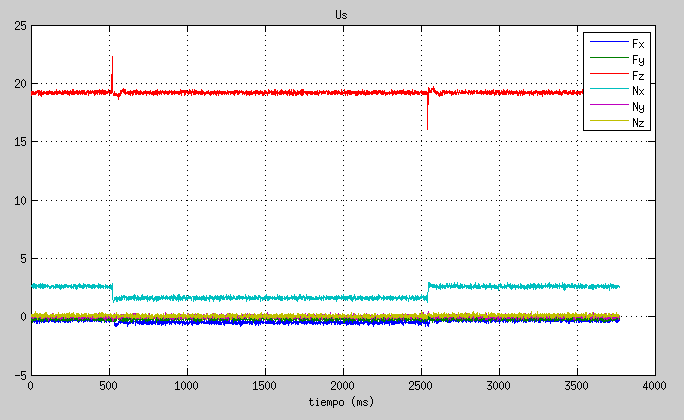
\includegraphics[scale=0.6]{Figuras/FTerror8}
\caption{Fuerza medida por el sensor fuerza par simulado, a 0.5kHz, aplicando 10Nm alrededor del eje $y$ .}
\label{fig:errorFTsensor8}
\end{figure}

Este aspecto es de gran importancia puesto que conlleva una incapacidad por parte del sistema de identificar este tipo de esfuerzos, hecho independiente del algoritmo empleado para la identificación de fuerzas externas, por lo que se tratará de evitar esta situación para analizar el comportamiento del observador. \par 

\end{itemize}

\section{Resultados de las simulaciones}

Salvando las dificultades mostradas en el apartado \ref{sec:dificultades}, se dispone a mostrar los resultados obtenidos en los distintos ensayos realizados. \par 

El código desarrollado puede consultarse en el Apéndice \ref{app:implemObservador}. En la presente sección se mostrarán los resultados obtenidos tras ejecutar el algoritmo del observador mostrado en el apartado \ref{sec:AlgoritObservador}. Se compararán además distintas situaciones simuladas con el fin de poder analizar más en profundidad las virtudes y defectos del algoritmo propuesto en el presente texto. \par 

Los ensayos que van a exponerse tendrán como objetivo intentar abarcar la mayor parte de las posibles situaciones existentes en la realidad, entre las cuales se van a considerar las siguientes:

\begin{enumerate}
\item Sin movimiento y sin fuerza externa.
\item Sin movimiento y aplicando fuerza externa.
\item Con movimiento y sin fuerza externa.
\item Combinando movimiento con fuerza externa.
\end{enumerate}

Ante todas estas posibilidades se estudiará la respuesta del observador tanto ante cargas estáticas como ante cargas variables en el tiempo. En todos los casos, si el sistema formado por el observador es estable, debería tender la estimación al estado real del sistema, puesto que la naturaleza recursiva del \emph{Filtro de Kalman} hace que converja hacia éste al aumentar el número de iteraciones del algoritmo. \par 

En primer lugar se analizará la estimación efectuada por el observador del estado del sistema en las cuatro situaciones enumeradas con anterioridad, y posteriormente se analizará la estimación de la fuerza externa aplicada. \par 

\subsection{Análisis de las estimaciones del estado}

En todos los casos se mostrará en las figuras una comparación entre el estado medido por los sensores $\boldsymbol{X}$ y el estimado por el observador $\boldsymbol{\hat{X}}$. Como se apreciará a continuación, las estimaciones efectuadas por el observador son muy cercanas a las reales en todos los casos en los que existe cierto nivel de ruido, no siendo así en aquellos en los que éste no exista. \par 

Para todos los casos posteriores, a excepción de aquellos en los que se especifique lo contrario, la frecuencia de adquisición de datos es de 500 Hz, y el ruido especificado para los sensores es de 0.1 de desviación típica para el sensor fuerza par, y de 0.01 para el resto (sensor inercial y odometría). \par 

Es preciso remarcar que el estado mostrado en las gráficas es el resultante tras efectuar un giro de 0.1 radianes alrededor del primer \acrshort{gdl}, \acrshort{sa}, con el fin de salvar el comportamiento extraño detectado en la posición inicial del sistema descrito en el apartado \ref{sec:dificultades}. \par 

Todos los ensayos mostrados presentan la dificultad inherente de la integración de las medidas de aceleración y velocidad, puesto que al aplicar la fuerza se produce un mínimo desplazamiento, el cual puede llegar a desviar la estimación a causa de la acumulación de errores en la integración. \par 

En la tabla \ref{tab:ensayos} pueden consultarse el número de ensayos realizados así como las características de dicho ensayo. \par 

\begin{table}
\centering
\begin{tabular}[c]{ c c c p{4.75cm} c }
\hline
\multicolumn{5}{c}{Ensayos efectuados} \\
\hline
Nº de Ensayo & Movimiento & Fuerza & Otras características & Figuras asociadas \\
\hline
1 & No & No &   & \ref{fig:smsf-X}, \ref{fig:smsf-Ue}\\
2 & No & Sí & 10 N en sentido positivo del eje $x$\footnotemark[1]. & \ref{fig:smcf-X}, \ref{fig:compfiltros}, \ref{fig:smcf-Fx} \\
3 & No & Sí & Rampa hasta 20 N en sentido positivo del eje $y$\footnotemark[1]. & \ref{fig:smcf-Fy} \\
4 & No & Sí & Escalones de 15 N en sentido negativo del eje $z$\footnotemark[1]. & \ref{fig:smcf-X-Fz}, \ref{fig:smcf-Fz} \\
5 & No & Sí & 5 Nm en sentido positivo del eje $x$\footnotemark[1]. & \ref{fig:smcf-Nx} \\
6 & No & Sí & 10 N en sentido negativo del eje $y$\footnotemark[1]. & \ref{fig:errorFTsensor8} \\
7 & No & Sí & Carga oscilante de 10Nm a -10Nm cada 500ms aplicadas alrededor del eje $z$\footnotemark[1]. & \ref{fig:smcf-X-Nz}, \ref{fig:smcf-X-Nz2}, \ref{fig:smcf-Nz} \\
8 & Sí & No & Movimiento alrededor de la articulación SA. & \ref{fig:cmsf-X-SA}, \ref{fig:cmsf-SA}, \ref{fig:cmsf-Y-SA} \\
9 & Sí & No & Movimiento alrededor de la articulación WR y SA. & \ref{fig:cmsf-X-WRSA}, \ref{fig:cmsf-X-WRSA2}, \ref{fig:cmsf-WRSA} \\
10 & Sí & No & Movimiento alrededor de la articulación SA sin controlador. & \ref{fig:cmsf-SAsc} \\
11 & Sí & No & Movimiento alrededor de la articulación SA con controlador a menor velocidad. & \ref{fig:cmsf-SAlento} \\
12 & Sí & No & Movimiento alrededor de la articulación WR y SA con controlador a menor velocidad. & \ref{fig:cmsf-WRSAlento} \\
13 & Sí & Sí & Movimiento alrededor de la articulación SA ejerciéndose una fuerza de -20 N a lo largo del eje $z$\footnotemark[1]. & \ref{fig:cmcf-X}, \ref{fig:cmcf-SA-Fz} \\
14 & Sí & Sí & Movimiento alrededor de la articulación SA ejerciéndose un momento de 7 Nm y -7 Nm alrededor del eje $z$\footnotemark[1]. & \ref{fig:cmcf-X}, \ref{fig:cmcf-SA-Nz} \\
15 & Sí & Sí & Movimiento alrededor de la articulación SA, sin controlador, ejerciéndose una fuerza de -20 N a lo largo del eje $z$\footnotemark[1]. & \ref{fig:cmcf-Xsc}, \ref{fig:cmcf-SAsc-Fz} \\
16 & Sí & Sí & Movimiento alrededor de la articulación SA, sin controlador, ejerciéndose un momento de 7 Nm y -7 Nm alrededor del eje $z$\footnotemark[1]. & \ref{fig:cmcf-Xsc}, \ref{fig:cmcf-SAsc-Nz} \\
\hline
\end{tabular}
\caption{Ensayos efectuados}
\label{tab:ensayos}
\end{table}

\footnotetext[1]{En todos los ensayos la fuerza es aplicada bajo el sistema de referencia móvil ligado al centro de masas del elemento terminal.}

\subsubsection{Sin movimiento y sin fuerza externa}

Tras lanzar la simulación, se observa que una vez fijo el extremo del robot, la estimación producida del estado del sistema es prácticamente idéntica al estado real del sistema, como bien puede apreciarse en la figura \ref{fig:smsf-X}. \par 

\begin{figure}[h!]
\centering
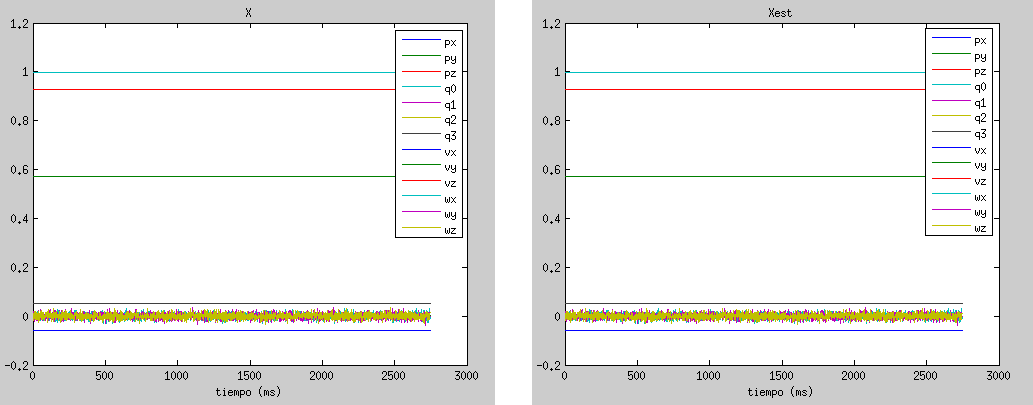
\includegraphics[scale=0.4]{Figuras/smsf-X}
\caption[Ensayo 1. Estimación del estado sin movimiento y sin fuerza]{Ensayo 1. Estimación del estado sin movimiento y sin fuerza. A la izquierda: estado medido por los sensores. A la derecha: estimación del estado.}
\label{fig:smsf-X}
\end{figure}

\subsubsection{Sin movimiento y con fuerza externa}

Con el fin de efectuar un análisis más detallado del comportamiento del observador, se aplicarán distintas fuerzas y momentos en distintas direcciones. \par 

\begin{figure}[h!]
\centering
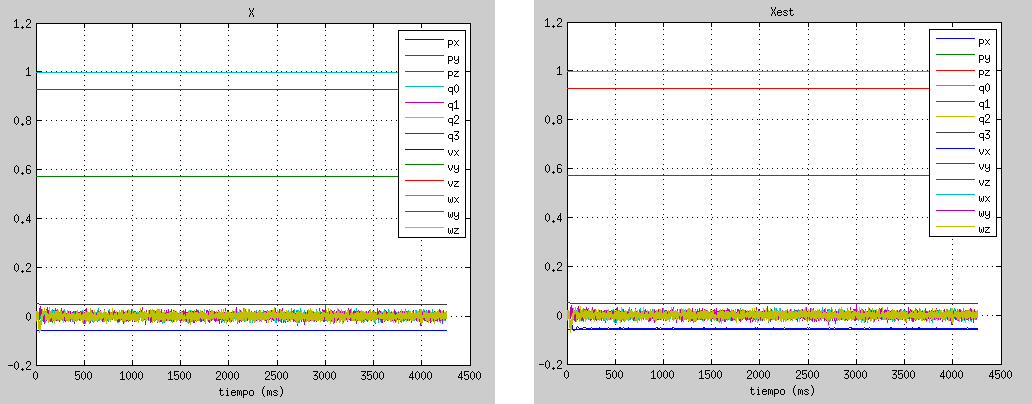
\includegraphics[scale=0.4]{Figuras/smcf-X}
\caption[Ensayo 2. Estimación del estado sin movimiento y con fuerza]{Ensayo 2. Estimación del estado sin movimiento y con fuerza: aplicando 10 N en sentido positivo del eje $x$. A la izquierda: estado medido por los sensores. A la derecha: estimación del estado.}
\label{fig:smcf-X}
\end{figure}

En la figura \ref{fig:smcf-X} puede apreciarse el resultado obtenido al aplicar una fuerza de 10 N en sentido positivo del eje $x$. Estos resultados son aplicables a todos los demás experimentos realizados, puesto que la ausencia de movimiento hace que todas las gráficas sean similares, exceptuando los casos descritos a continuación. \par 

\begin{itemize}

\item \textbf{\emph{Ensayo 4}}: Escalones intermitentes de -15 N de amplitud en dirección del eje $z$ móvil.

\begin{figure}[h!]
\centering
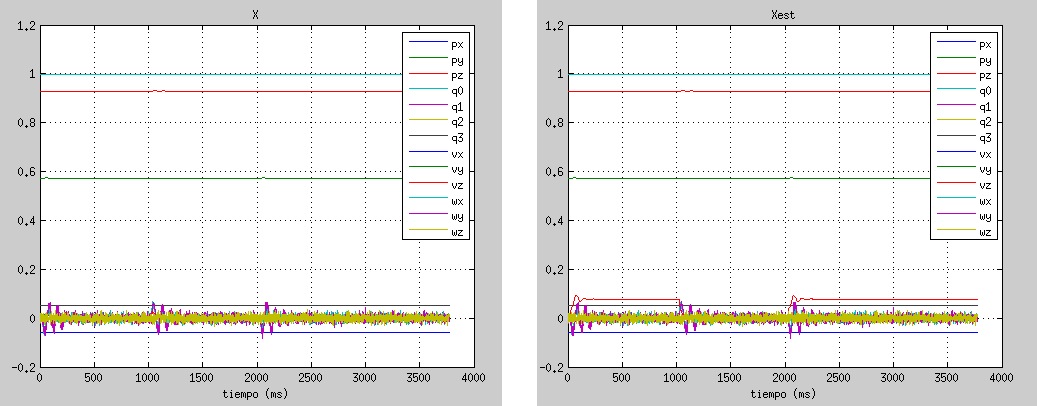
\includegraphics[scale=0.4]{Figuras/smcf-X-Fz}
\caption[Ensayo 4. Estimación del estado sin movimiento y con fuerza]{Ensayo 4. Estimación del estado sin movimiento y con fuerza: se ejercen escalones de 15 N en sentido negativo del eje $z$. A la izquierda: estado medido por los sensores. A la derecha: estimación del estado.}
\label{fig:smcf-X-Fz}
\end{figure}

En este caso, como muestra la figura \ref{fig:smcf-X-Fz}, la estimación se desvía del estado medido por los sensores debido a la fuerza externa aplicada al sistema, lo cual no quiere decir que la estimación no sea aceptable, sino que al no estar incluida la fuerza externa en el modelo, esta situación es indispensable para una correcta estimación de la misma. \par 

\item \textbf{\emph{Ensayo 7}}: Sin movimiento se aplica un momento de 10 Nm alrededor del eje $z$ durante 500 ms y de -10 Nm durante los 500 ms siguientes, siendo periódica esta secuencia a lo largo del tiempo. \par 

\begin{figure}[h!]
\centering
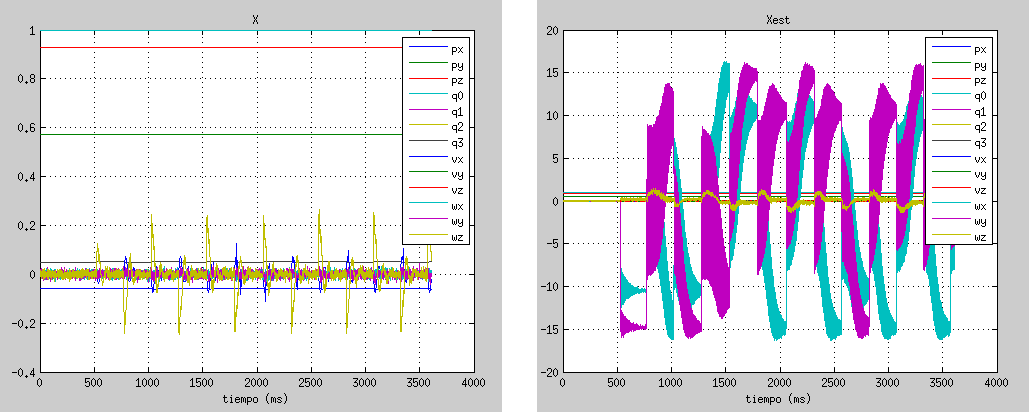
\includegraphics[scale=0.4]{Figuras/smcf-X-Nz}
\caption[Ensayo 7. Estimación del estado sin movimiento y con fuerza]{Ensayo 7. Estimación del estado sin movimiento y con fuerza: se ejerce una carga oscilante de 10Nm a -10Nm cada 500ms aplicadas alrededor del eje $z$. A la izquierda: estado medido por los sensores. A la derecha: estimación del estado.}
\label{fig:smcf-X-Nz}
\end{figure}

En vistas a estos resultados y los obtenidos en el ensayo 9 (ver figura \ref{fig:cmsf-X-WRSA}), se propone aumentar un orden de magnitud la desviación típica especificada en el algoritmo para los valores de $\boldsymbol{\dot{\omega}}$ (hasta ahora se habían establecido en 1) hasta 100. \par 

Una vez modificados estos parámetros se obtiene una estimación como la mostrada en la figura \ref{fig:smcf-X-Nz2}, en la cual se aprecia la notoria mejoría con respecto a la obtenida en la figura \ref{fig:smcf-X-Nz}. \par 

\begin{figure}[h!]
\centering
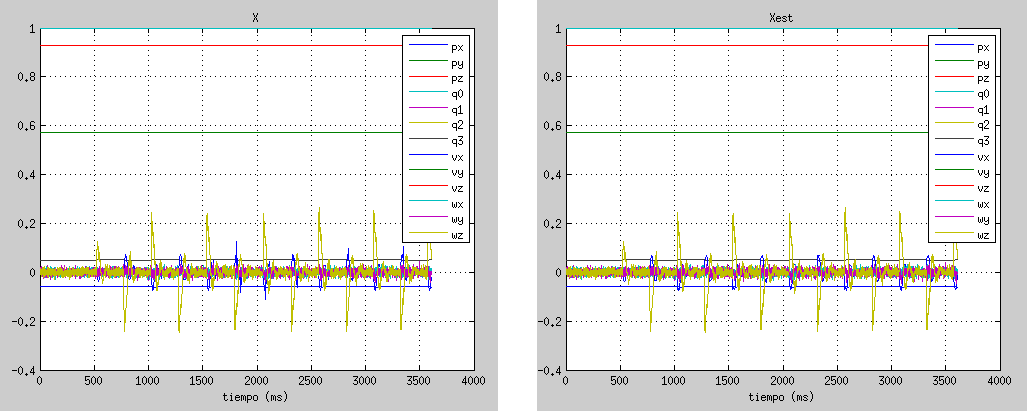
\includegraphics[scale=0.4]{Figuras/smcf-X-Nz2}
\caption[Ensayo 7. Estimación del estado corregida, sin movimiento y con fuerza]{Ensayo 7. Estimación del estado corregida, sin movimiento y con fuerza: se ejerce una carga oscilante de 10Nm a -10Nm cada 500ms aplicadas alrededor del eje $z$. A la izquierda: estado medido por los sensores. A la derecha: estimación del estado.}
\label{fig:smcf-X-Nz2}
\end{figure}

\end{itemize}

\subsubsection{Con movimiento y sin fuerza externa}

Los movimientos que se van a efectuar en este apartado intentarán abarcar todos los ejes posibles de rotación y desplazamientos en los tres ejes primarios, con el fin de probar la efectividad del observador en todos ellos. \par 

\begin{itemize}

\item \textbf{\emph{Ensayo 8}}: Movimiento de 0.5 radianes alrededor de la articulación \acrshort{sa}, es decir, alrededor del primer \acrshort{gdl} (figura \ref{fig:cmsf-X-SA}).

\begin{figure}[h!]
\centering
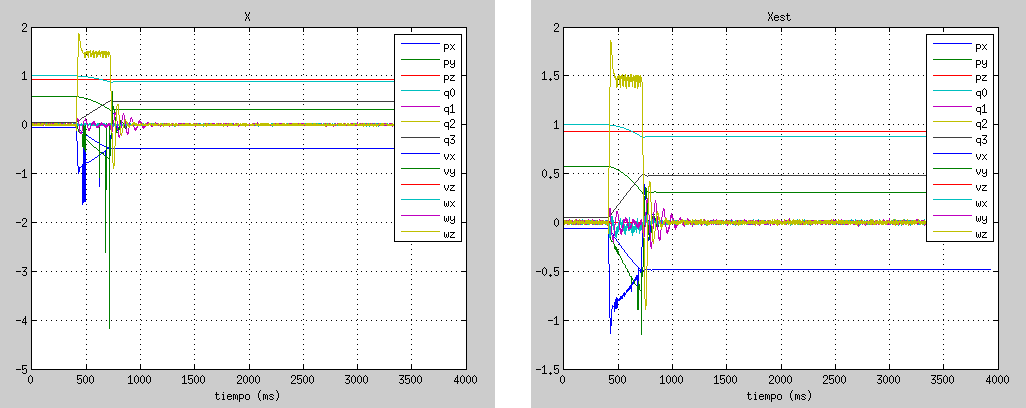
\includegraphics[scale=0.4]{Figuras/cmsf-X-SA}
\caption[Ensayo 8. Estimación del estado con movimiento y sin fuerza]{Ensayo 8. Estimación del estado con movimiento y sin fuerza: se efectúa un movimiento alrededor de la articulación \acrshort{sa}. A la izquierda: estado medido por los sensores. A la derecha: estimación del estado.}
\label{fig:cmsf-X-SA}
\end{figure}

En la figura \ref{fig:cmsf-X-SA} pueden apreciarse claramente los instantes en los que se produce el movimiento. En las medidas del sensor puede observarse en ciertos instantes valores anormales, variaciones excesivamente bruscas en la velocidad lineal medida ($v_x$ y $v_y$). En cambio en la estimación no aparecen estos valores alejados al de la realidad. \par 

Una vez finalizado el movimiento ambas gráficas muestran los mismos valores para todas sus variables, por lo que las estimaciones son idénticas en régimen permanente. En régimen transitorio, para este caso concreto, también son acertadas las estimaciones del estado efectuadas por el observador. \par 

\item \textbf{\emph{Ensayo 9}}: Movimiento, en primer lugar, de 1 radian alrededor de la articulación \acrshort{wr}, el sexto \acrshort{gdl} del manipulador, y posteriormente de 0.5 radianes alrededor de \acrshort{sa}. \par 

\begin{figure}[h!]
\centering
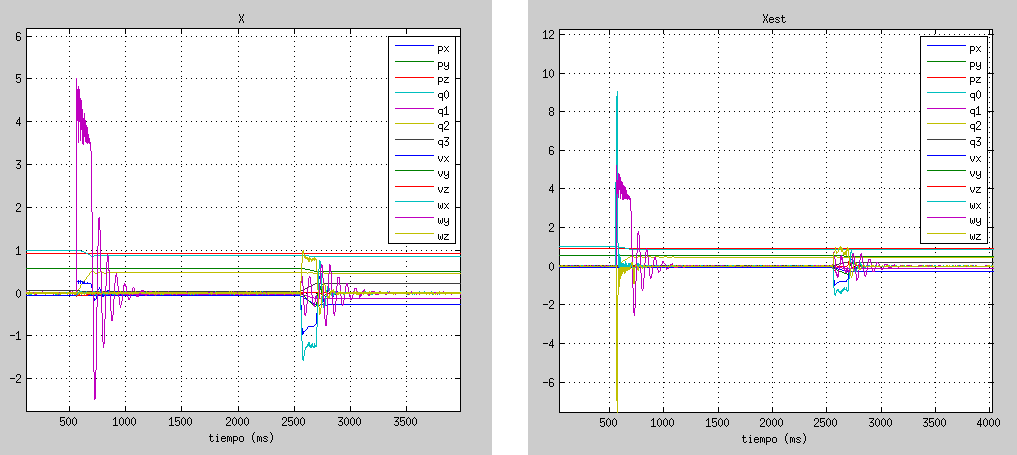
\includegraphics[scale=0.4]{Figuras/cmsf-X-WRSA}
\caption[Ensayo 9. Estimación del estado con movimiento y sin fuerza]{Ensayo 9. Estimación del estado con movimiento y sin fuerza: se efectúa un movimiento alrededor de la articulación \acrshort{wr} y \acrshort{sa}. A la izquierda: estado medido por los sensores. A la derecha: estimación del estado.}
\label{fig:cmsf-X-WRSA}
\end{figure}

En la figura \ref{fig:cmsf-X-WRSA} puede apreciarse una notoria desviación de la estimación del estado al iniciarse el primer movimiento para valores de la velocidad angular ($\omega_x$ y $\omega_z$). En cambio la estimación producida en el segundo movimiento es prácticamente idéntica a la real. \par 

\begin{figure}[h!]
\centering
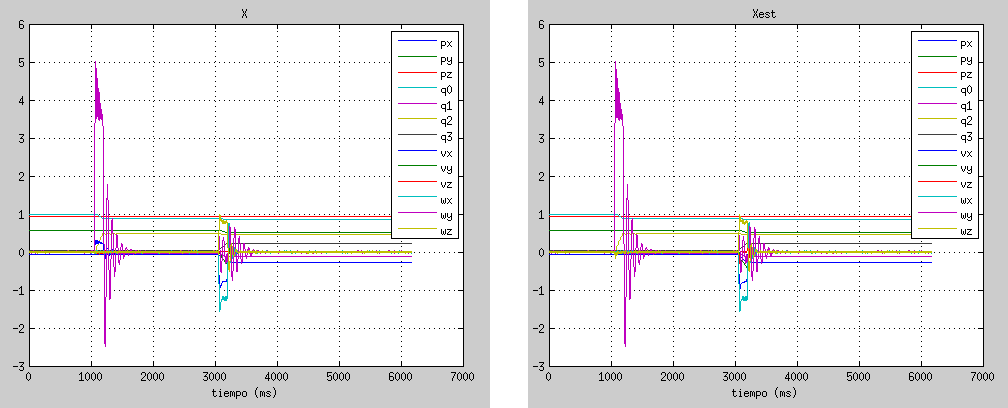
\includegraphics[scale=0.4]{Figuras/cmsf-X-WRSA2}
\caption[Ensayo 9. Estimación del estado corregida, con movimiento y sin fuerza]{Ensayo 9. Estimación del estado corregida, con movimiento y sin fuerza: se efectúa un movimiento alrededor de la articulación \acrshort{wr} y \acrshort{sa}. A la izquierda: estado medido por los sensores. A la derecha: estimación del estado.}
\label{fig:cmsf-X-WRSA2}
\end{figure}

Una vez efectuada la modificación especificada en el ensayo 7, se obtiene una estimación mucho más cercana a la real medida por los sensores, como muestra la figura \ref{fig:cmsf-X-WRSA2}, por lo que esta última es la considerada al efectuar las evaluaciones del algoritmo observador y estimador de fuerzas externas. \par 

\end{itemize}

\subsubsection{Con movimiento y con fuerza externa}

Esta situación es la más compleja a la que puede enfrentarse el algoritmo estimador de fuerzas externas, puesto que es en el que interviene un mayor número de factores simultáneamente. \par 

\begin{itemize}

\item \textbf{\emph{Ensayos 13 y 14}}: Movimiento alrededor del primer grado de libertad (articulación \acrshort{sa}) mientras el cual se aplica una fuerza de -20 N en $z$ (ensayo 13) o un momento de 7 Nm y -7 Nm alrededor del eje $z$ (ensayo 15). En ambos ensayos el movimiento es efectuado con el controlador del manipulador (figura \ref{fig:cmcf-X}).

\begin{figure}[h!]
\centering
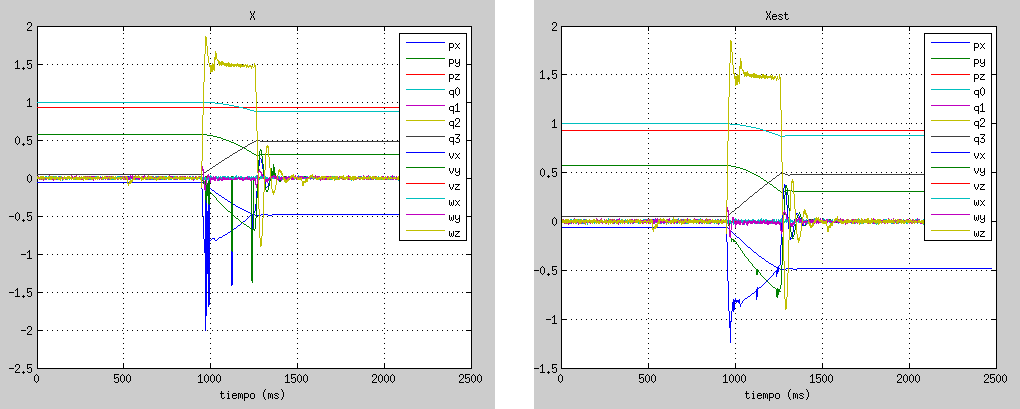
\includegraphics[scale=0.4]{Figuras/cmcf-X}
\caption[Ensayos 13 y 14. Estimación del estado con movimiento y con fuerza]{Ensayos 13 y 14. Estimación del estado con movimiento y con fuerza. A la izquierda: estado medido por los sensores. A la derecha: estimación del estado.}
\label{fig:cmcf-X}
\end{figure}

\item \textbf{\emph{Ensayos 15 y 16}}: Movimiento alrededor del primer grado de libertad (articulación \acrshort{sa}) mientras el cual se aplica una fuerza de -20 N en $z$ (ensayo 13) o un momento de 7 Nm y -7 Nm alrededor del eje $z$ (ensayo 15). En ambos ensayos el movimiento es efectuado sin uso del controlador del manipulador (figura \ref{fig:cmcf-Xsc}).

\begin{figure}[h!]
\centering
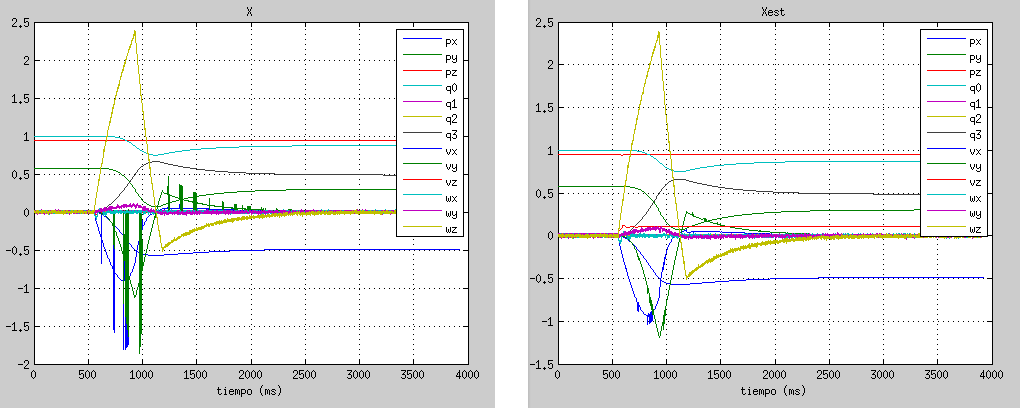
\includegraphics[scale=0.4]{Figuras/cmcf-Xsc}
\caption[Ensayo 15 y 16. Estimación del estado con movimiento con fuerza]{Ensayos 15 y 16. Estimación del estado con movimiento con fuerza. A la izquierda: estado medido por los sensores. A la derecha: estimación del estado.}
\label{fig:cmcf-Xsc}
\end{figure}

\end{itemize}

\subsection{Análisis de las estimaciones de la fuerza externa}

Debido a que la fuerza estimada por el algoritmo detallado en el anterior capítulo presenta una componente debida al ruido, como se muestra en la expresión \ref{eq:estimador-ruido}, es preciso efectuar un filtrado de estos resultados. \par 

Considerando constantes las desviaciones típicas del ruido de los sensores, el ruido en las estimaciones también será constante, puesto que la matriz $D_E$ también lo es. Por tanto se propone el uso de un filtro de paso bajo o \acrshort{lpf} (del inglés \emph{Low Pass Filter}), el cual filtrará en gran medida todas aquellas componentes de frecuencia superior a la de corte. \par 

\noindent
El algoritmo empleado para implementar el filtro de paso bajo en tiempo real es el siguiente:

\begin{equation}
	OUT_k = OUT_{k-1} + \alpha(IN_k - OUT_{k-1})
\end{equation} \\
\noindent
donde $\alpha$ es un parámetro constante que determina la frecuencia de corte del filtro, $OUT$ representa el valor de salida del filtro (estimación filtrada), e $IN$ el valor de entrada (estimación sin filtrar). \par 

Es preciso en primer lugar, establecer la frecuencia de corte correcta para obtener unos resultados suficientemente cercanos a la realidad pero libres de ruido. Una disminución de la frecuencia de corte supone un filtrado de un mayor rango de frecuencias en la señal, pero presenta la contrapartida de que hace más lenta la respuesta, por lo que es preciso alcanzar un compromiso entre un filtrado de un mayor rango de frecuencias en la señal y la rapidez de respuesta del estimador. \par 

\begin{figure}[h!]
\centering
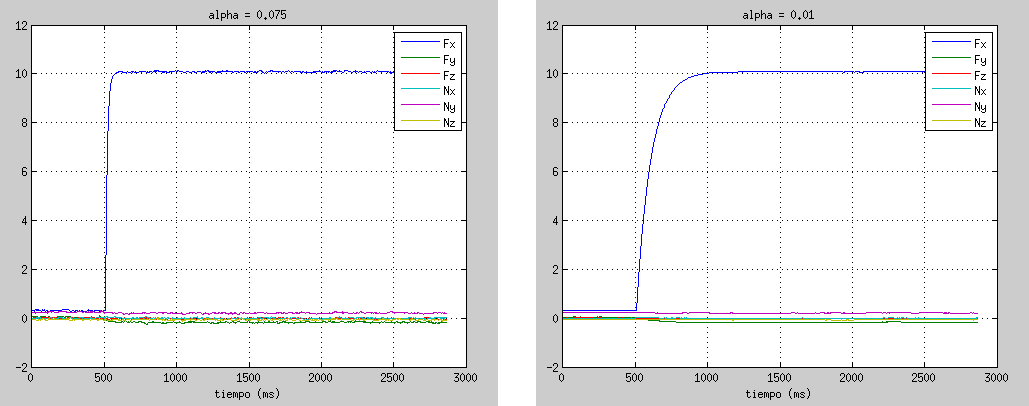
\includegraphics[scale=0.4]{Figuras/compfiltros}
\caption[Ensayo 2. Fuerza estimada sin movimiento y con fuerza]{Ensayo 2. Sin movimiento y con fuerza: se ejercen 10 N en sentido positivo del eje $x$. A la izquierda: fuerza externa estimada filtrada con $\alpha = 0.075$. A la derecha: fuerza externa estimada filtrada con $\alpha = 0.01$.}
\label{fig:compfiltros}
\end{figure}

Efectuando distintas pruebas se ha llegado a la conclusión de que el uso de un parámetro $\alpha$ de 0.075 se obtienen resultados satisfactorios. En la figura \ref{fig:compfiltros} se puede apreciar la diferencia entre un valor de $\alpha = 0.075$ a la izquierda y otro de $\alpha = 0.01$ a la derecha, aplicados a las estimaciones producidas de la fuerza externa del ensayo 2. \par 

Se mostrará en todas las gráficas de la actual sección una comparación entre la estimación directa obtenida mediante el estimador y la resultante tras el proceso de filtrado. \par 

\subsubsection{Sin movimiento y sin fuerza externa}

El resultado esperado en este ensayo es el de una fuerza y momentos nulos. La obtención de estos resultados supondría una cancelación efectiva de la componente de la fuerza debida a la aceleración de la gravedad, es decir, una compensación estática. \par 

Para evitar las dificultades encontradas y mencionadas en el apartado \ref{sec:dificultades}, se ha empleado una frecuencia de adquisición de datos de 500 Hz. \par 

\begin{figure}[h!]
\centering
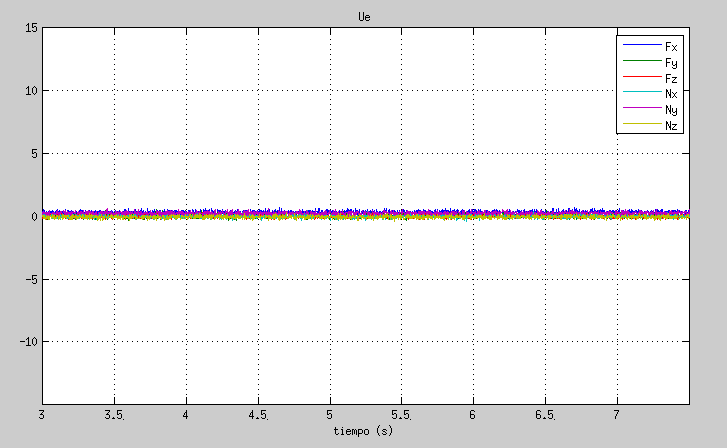
\includegraphics[scale=0.55]{Figuras/smsf-Ue}
\caption[Ensayo 1. Fuerza estimada sin movimiento y sin fuerza]{Ensayo 1. Fuerza estimada sin y movimiento sin fuerza.}
\label{fig:smsf-Ue}
\end{figure}

Puede apreciarse en la figura \ref{fig:smsf-Ue} una correcta compensación estática efectuada por el algoritmo estimador de fuerzas externas, en la que aparece fuerza y momento nulo en todo momento en todas las componentes mostradas en la figura. \par  

\subsubsection{Sin movimiento y con fuerza externa}

Con estos ensayos se pretende verificar la efectividad del estimador sin movimiento alguno del manipulador, con lo que se comprobará la ganancia estática del algoritmo, es decir, que la relación entre la carga aplicada y la estimada sea la unidad. \par 

Se analizará el comportamiento del algoritmo ante cargas variables en el tiempo, aspecto importante, puesto que en la mayor parte de las aplicaciones reales se producirá esta situación. \par 

\begin{itemize}
\item \textbf{\emph{Ensayo 2}}: Sin movimiento se aplica un escalón de 10 N en sentido positivo del eje $x$ (figura \ref{fig:smcf-Fx}).

\begin{figure}[h!]
\centering
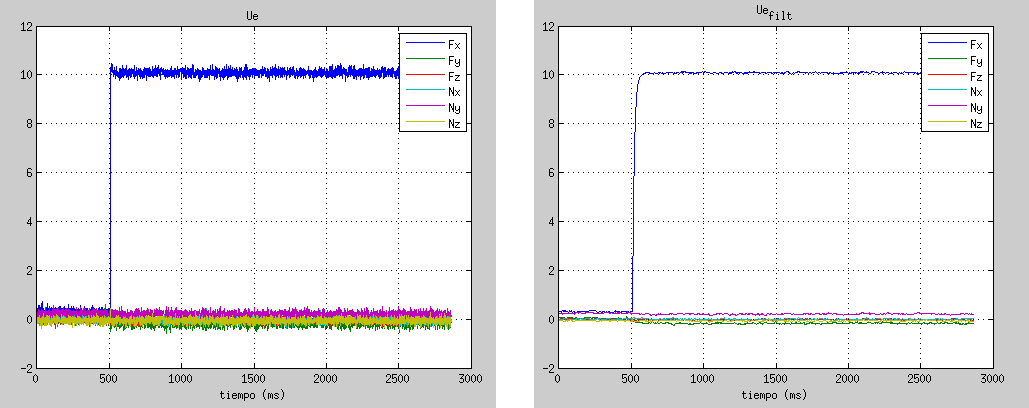
\includegraphics[scale=0.4]{Figuras/smcf-Fx}
\caption[Ensayo 2. Fuerza estimada sin movimiento y con fuerza]{Ensayo 2. Fuerza estimada sin movimiento y con fuerza: se ejercen 10 N en sentido positivo del eje $x$. A la izquierda: fuerza externa estimada por el algoritmo. A la derecha: fuerza estimada filtrada.}
\label{fig:smcf-Fx}
\end{figure}

Efectuando la modificación mencionada en \ref{sec:dificultades} acerca de la fuerza residual en dirección del eje $y$ móvil, se obtiene la respuesta mostrada en la figura \ref{fig:smcf-Fx}, en la cual puede apreciarse una respuesta inmediata del estimador ante la aplicación del escalón de 10 N. \par 

Por un lado puede observarse la eliminación de la componente de la gravedad, puesto que no aparece reflejada ninguna fuerza en dirección del eje $z$, y además de la debida a la inercia, puesto que al ejercer la fuerza se produce un pequeño desplazamiento que es detenido por el controlador del manipulador (puede observarse esa pequeña oscilación en la figura \ref{fig:errorFTsensor6}, donde se muestra la fuerza medida por el sensor en un ensayo similar). De esta manera la respuesta obtenida es el escalón ejercido. \par 

\item \textbf{\emph{Ensayo 3}}: Sin movimiento se ejerce una rampa hasta alcanzar los 20 N en sentido positivo del eje $y$ (figura \ref{fig:smcf-Fy}).

\begin{figure}[h!]
\centering
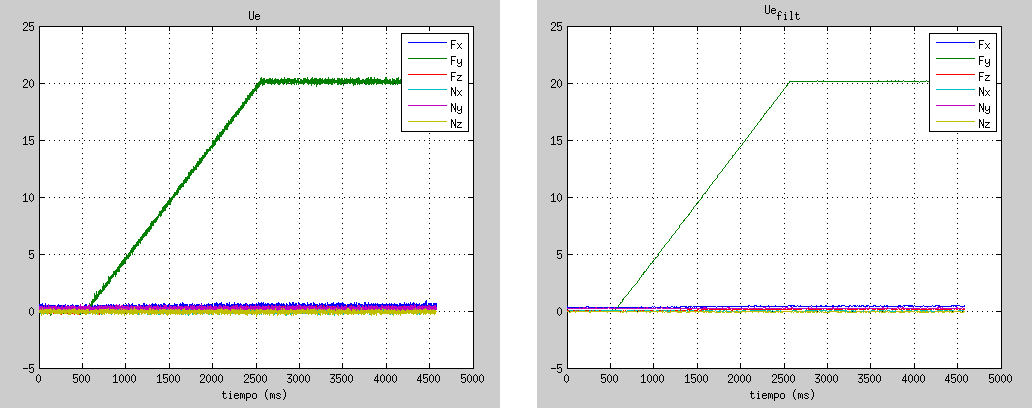
\includegraphics[scale=0.4]{Figuras/smcf-Fy}
\caption[Ensayo 3. Fuerza estimada sin movimiento y con fuerza]{Ensayo 3. Fuerza estimada sin movimiento y con fuerza: se ejerce una rampa hasta 20 N en sentido positivo del eje $y$. A la izquierda: fuerza externa estimada por el algoritmo. A la derecha: fuerza estimada filtrada.}
\label{fig:smcf-Fy}
\end{figure}

Al igual que en el caso anterior ha sido necesaria una compensación de la fuerza residual mencionada en \ref{sec:dificultades}, ejerciendo una fuerza en dirección $x$ diez veces inferior a la ejercida en $y$. \par 

Puede observarse igualmente un correcto funcionamiento del estimador, obteniéndose una respuesta idéntica a la fuerza externa aplicada en este ensayo. \par 

\item \textbf{\emph{Ensayo 4}}: Sin movimiento se ejerce de manera intermitente dos escalones de -15 N de amplitud en dirección del eje $z$ (figura \ref{fig:smcf-Fz}).

\begin{figure}[h!]
\centering
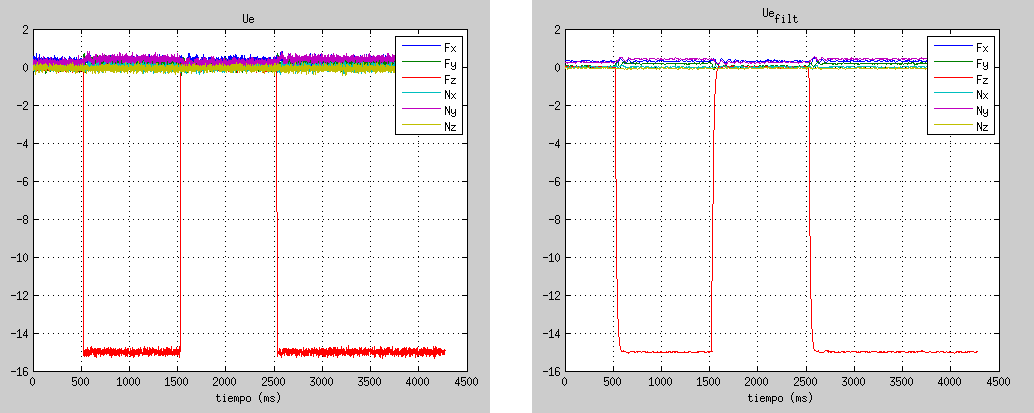
\includegraphics[scale=0.4]{Figuras/smcf-Fz}
\caption[Ensayo 4. Fuerza estimada sin movimiento y con fuerza]{Ensayo 4. Fuerza estimada sin movimiento y con fuerza: se ejercen escalones de 15 N en sentido negativo del eje $z$. A la izquierda: fuerza externa estimada por el algoritmo. A la derecha: fuerza estimada filtrada.}
\label{fig:smcf-Fz}
\end{figure}

La respuesta obtenida en la figura \ref{fig:smcf-Fz} puede asemejarse a la existente al someter al manipulador a un peso en el elemento terminal, como puede suceder en la sujeción de un objeto. \par 

Como en los casos mostrados con anterioridad, la estimación efectuada por el algoritmo propuesto es similar a la aplicada al elemento terminal, en la que se ha efectuado una compensación estática y dinámica de las fuerzas y momentos medidos por el sensor fuerza par. \par 

\item \textbf{\emph{Ensayo 5}}: Sin movimiento se aplica un momento en dirección del eje $x$ móvil de amplitud -5 Nm, referido al sistema de referencia ligado al centro de masas del elemento terminal (figura \ref{fig:smcf-Nx}). \par 

\begin{figure}[h!]
\centering
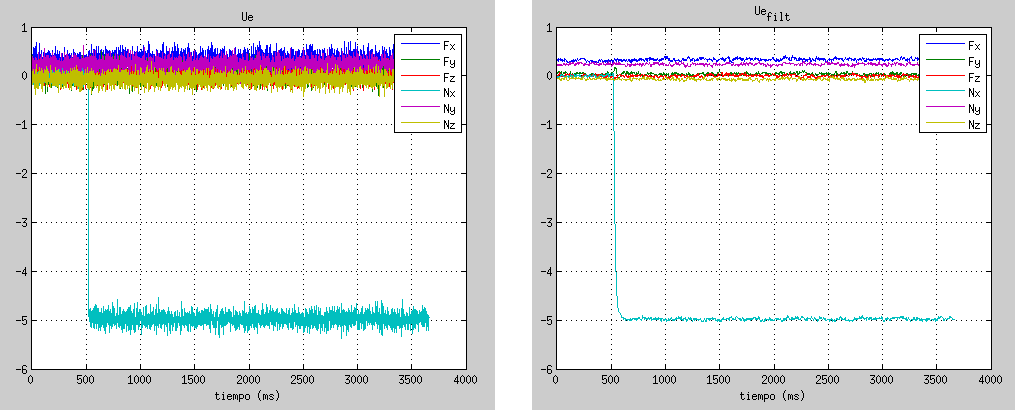
\includegraphics[scale=0.4]{Figuras/smcf-Nx}
\caption[Ensayo 5. Fuerza estimada sin movimiento y con fuerza]{Ensayo 5. Fuerza estimada sin movimiento y con fuerza: se ejerce un escalón de 5 Nm en sentido positivo del eje $x$. A la izquierda: fuerza externa estimada por el algoritmo. A la derecha: fuerza estimada filtrada.}
\label{fig:smcf-Nx}
\end{figure}

Puede observarse una correcta estimación del momento aplicado en la figura \ref{fig:smcf-Nx}. \par 

\item \textbf{\emph{Ensayo 6}}: Sin existencia de movimiento alguno se aplica un momento en dirección del eje $y$ móvil. \par 

Como se mencionó en el apartado de dificultades encontradas \ref{sec:dificultades}, ante esta situación el sistema no es capaz de identificar un momento aplicado en este sentido, por lo que la fuerza externa estimada no refleja la realidad a la que se encuentra sometida el sistema. \par 

La fuerza medida por el sensor es la representada en la figura \ref{fig:errorFTsensor8}, en la cual se observa que no existe componente alguna del momento alrededor del eje $y$ móvil, por lo que la estimación que se obtendría al ejecutar el algoritmo es distinta a la fuerza aplicada externamente. \par 

\item \textbf{\emph{Ensayo 7}}: Sin movimiento se aplica un momento de 10 Nm alrededor del eje $z$ durante 500 ms y de -10 Nm durante los 500 ms siguientes, siendo periódica esta secuencia a lo largo del tiempo. \par 

\begin{figure}[h!]
\centering
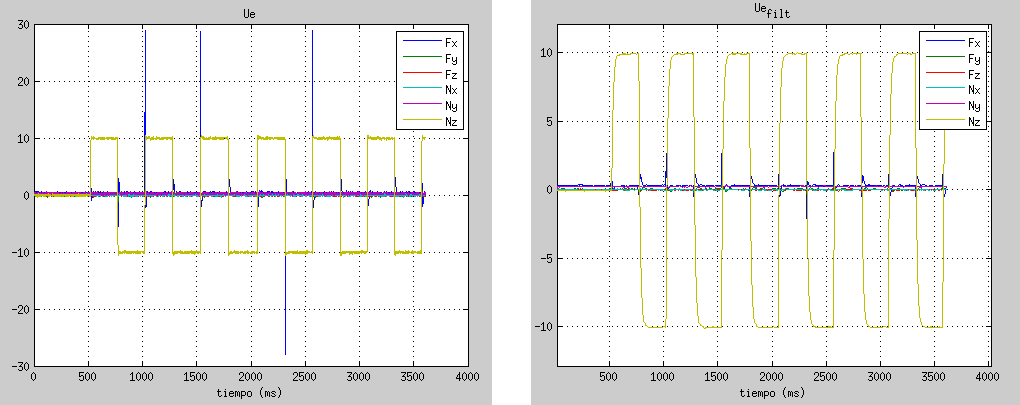
\includegraphics[scale=0.4]{Figuras/smcf-Nz}
\caption[Ensayo 7. Fuerza estimada sin movimiento y con fuerza]{Ensayo 7. Fuerza estimada sin movimiento y con fuerza: se ejerce una carga oscilante de 10Nm a -10Nm cada 500ms aplicadas alrededor del eje $z$. A la izquierda: fuerza externa estimada por el algoritmo. A la derecha: fuerza estimada filtrada.}
\label{fig:smcf-Nz}
\end{figure}
\end{itemize}

Pueden observarse ciertos valores medidos de la fuerza $F_x$ anormales, semejantes a los mostrados en la sección \ref{sec:dificultades}. A excepción de estos valores se puede apreciar una estimación muy acercada al momento aplicado. \par 

Tras efectuar un filtrado de la estimación estos valores anormales reducen su amplitud en comparación con la estimación inicial. \par 

\subsubsection{Con movimiento y sin fuerza externa}

En esta situación se busca verificar la capacidad del estimador de efectuar una compensación dinámica de las fuerzas medidas por el sensor fuerza par. Con cancelación dinámica se hace referencia a la identificación y separación de las componentes debidas al movimiento e inercia del manipulador. \par 

\begin{itemize}
\item \textbf{\emph{Ensayo 8}}: Se efectúa un giro de 1 radián alrededor del primer grado de libertad: la articulación \acrshort{sa} (figura \ref{fig:cmsf-SA}). \par 

\begin{figure}[h!]
\centering
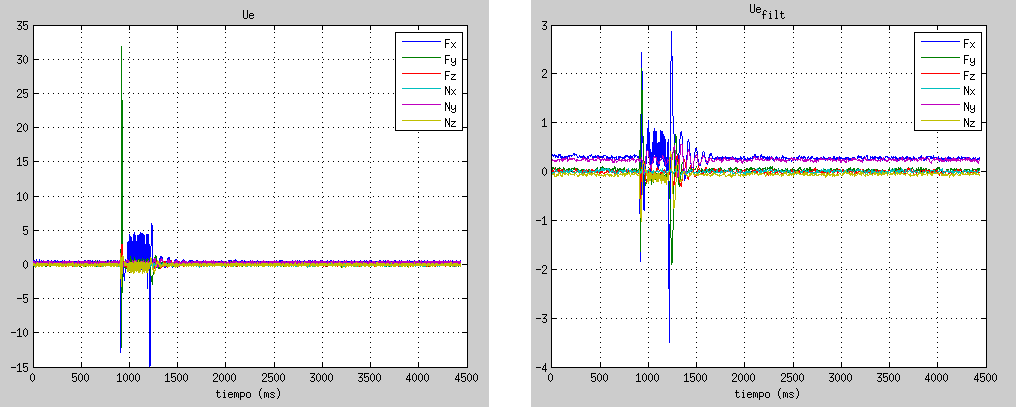
\includegraphics[scale=0.4]{Figuras/cmsf-SA}
\caption[Ensayo 8. Fuerza estimada con movimiento y sin fuerza]{Ensayo 8. Fuerza estimada con movimiento sin fuerza: se efectúa un movimiento alrededor de la articulación \acrshort{sa}. A la izquierda: fuerza externa estimada por el algoritmo. A la derecha: fuerza estimada filtrada.}
\label{fig:cmsf-SA}
\end{figure}

Puede observarse que la estimación no es la adecuada, debiendo ser la fuerza externa estimada nula en todo momento, debido a que únicamente se ha efectuado un movimiento con el manipulador. Es preciso por tanto efectuar un análisis más exhaustivo de la situación. \par 

En la figura \ref{fig:cmsf-Y-SA} puede observarse que la diferencia existente entre la fuerza externa estimada y la real es debida a la gran disparidad apreciable en la componente $\dot{\hat{\omega}}_x$. \par 

\begin{figure}[h!]
\centering
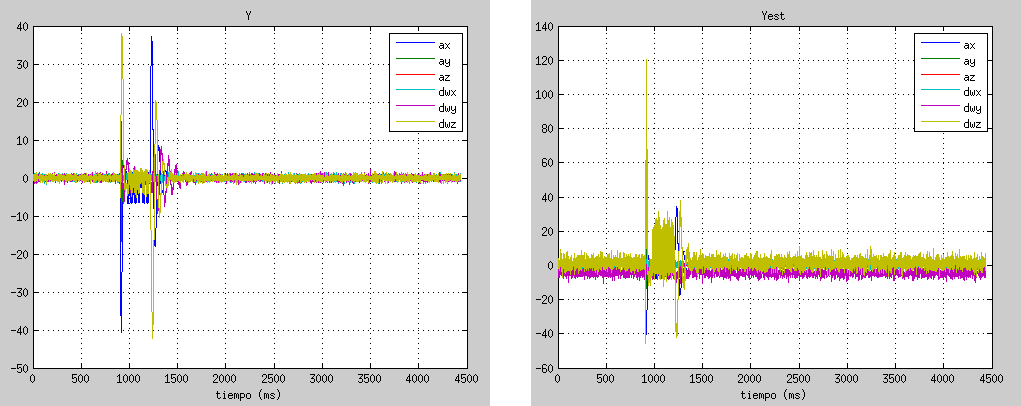
\includegraphics[scale=0.4]{Figuras/cmsf-Y-SA}
\caption[Ensayo 8. Vector de salida estimado con movimiento y sin fuerza.]{Ensayo 8. Vector de salida estimado con movimiento y sin fuerza: se efectúa un movimiento alrededor de la articulación \acrshort{sa}. A la izquierda: salida medida por los sensores. A la derecha: estimación de la salida.}
\label{fig:cmsf-Y-SA}
\end{figure}

Esta diferencia está causada por la gran sensibilidad existente en $\boldsymbol{\dot{\hat{\omega}}}$ a causa del factor por el que se multiplica dicha componente en el algoritmo observador, el cual es cercano a 30, por lo que una pequeña variación en los momentos medidos por el sensor fuerza par provoca una gran desviación en la estimación de la fuerza externa. \par 

\item \textbf{\emph{Ensayo 9}}: Se efectúa un giro de 1 radián alrededor del último grado de libertad: la articulación \acrshort{wr}, y posteriormente uno de 0.5 radianes alrededor del primer grado de libertad: la articulación \acrshort{sa} (figura \ref{fig:cmsf-WRSA}). \par 

\begin{figure}[h!]
\centering
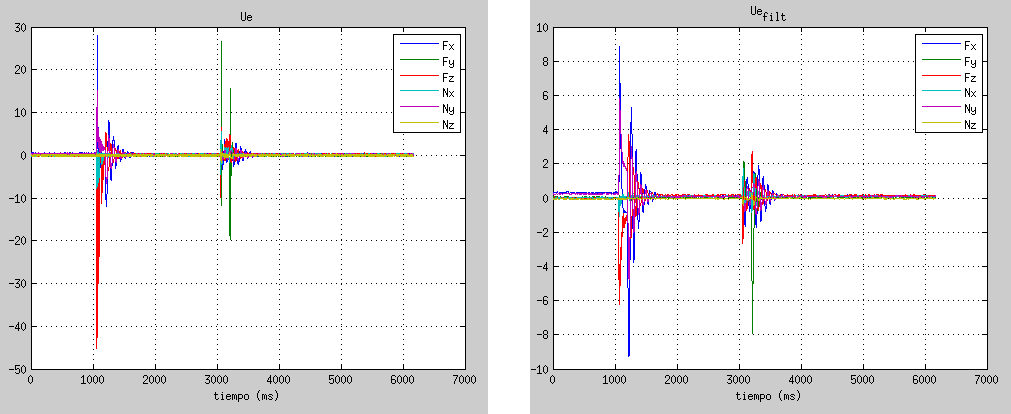
\includegraphics[scale=0.4]{Figuras/cmsf-WRSA}
\caption[Ensayo 9. Fuerza estimada con movimiento y sin fuerza]{Ensayo 9. Fuerza estimada con movimiento y sin fuerza: se efectúa un movimiento alrededor de la articulación \acrshort{wr} y \acrshort{sa}. A la izquierda: fuerza externa estimada por el algoritmo. A la derecha: fuerza estimada filtrada.}
\label{fig:cmsf-WRSA}
\end{figure}

Pueden apreciarse, al igual que sucedía en el ensayo anterior, los instantes de tiempo en los que se está produciendo el desplazamiento del elemento terminal, por lo que la compensación dinámica no es lo suficientemente acertada. \par 

\item \textbf{\emph{Ensayo 10}}: Movimiento alrededor de la articulación \acrshort{sa} sin uso del controlador del manipulador (figura \ref{fig:cmsf-SAsc}) sin ejercer fuerza externa alguna sobre el elemento terminal.

Debido a las bruscas aceleraciones inducidas en el elemento terminal a causa del control de posición empleado en el controlador del manipulador, se propone la alternativa de efectuar un movimiento sin emplear dicho controlador para verificar la efectividad del algoritmo estimador en este caso. \par 

\begin{figure}[h!]
\centering
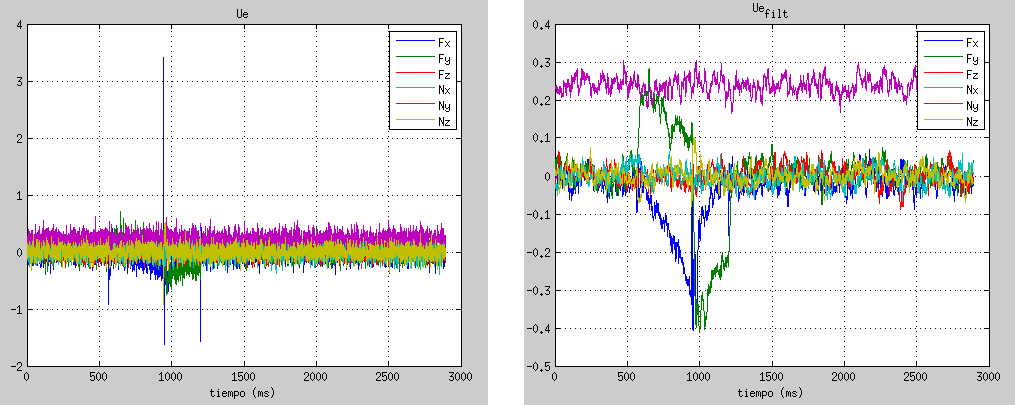
\includegraphics[scale=0.4]{Figuras/cmsf-SAsc}
\caption[Ensayo 10. Fuerza estimada con movimiento y sin fuerza]{Ensayo 10. Fuerza estimada con movimiento y sin fuerza: se efectúa un movimiento alrededor de la articulación \acrshort{sa} sin controlador. A la izquierda: fuerza externa estimada por el algoritmo. A la derecha: fuerza estimada filtrada.}
\label{fig:cmsf-SAsc}
\end{figure}

Este movimiento se consigue inhabilitando la acción del controlador para la articulación \acrshort{sa}, y ejerciendo un momento externo alrededor del eje $z$ del sistema de referencia fijo sobre la base del manipulador. Esto provoca un giro alrededor del primer grado de libertad, sin ejercer fuerza externa al sistema estudiado en el texto. \par 

En el presente ensayo se aplica un momento de 20 Nm alrededor del eje $z$ durante 750 ms y seguidamente -20 Nm durante 750 ms para detener el movimiento. Puede observarse el resultado obtenido por el estimador en la figura \ref{fig:cmsf-SAsc}. \par 

Se aprecia que la estimación en este ensayo es mucho más acercada a la situación real que en el resto de ensayos en los que se ha efectuado algún movimiento con el manipulador. \par 

Puede observarse, además, una pequeña desviación existente en las fuerzas estimadas: aparece un momento no nulo alrededor del eje $y$, del orden de 0.2Nm, el cual debería ser nulo. Esta situación pone de manifiesto que la cancelación estática no es perfecta, sino que existe una pequeña componente residual, debida a una imprecisión en la determinación de las propiedades físicas como la matriz de inercia, la masa o los vectores de posición entre los distintos sistemas de referencia. \par 

\item \textbf{\emph{Ensayo 11}}: Se efectúa un giro de 1 radián alrededor del primer grado de libertad: la articulación \acrshort{sa}, a velocidad reducida (figura \ref{fig:cmsf-SAlento}). \par 

\begin{figure}[h!]
\centering
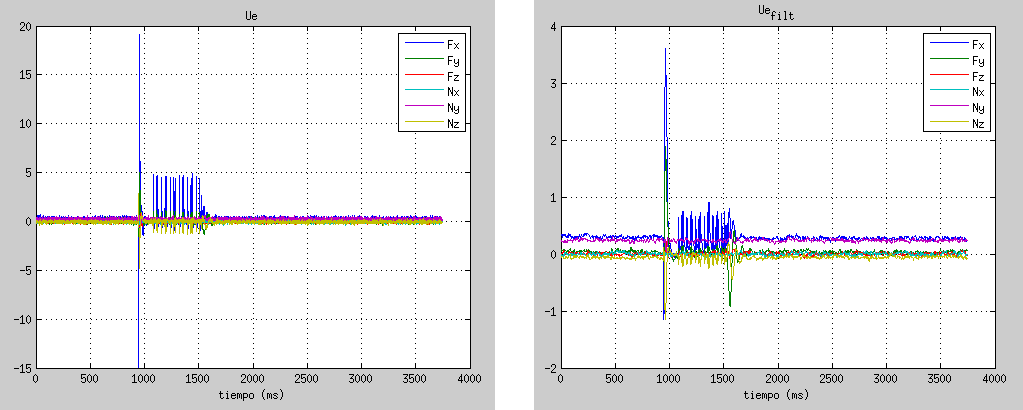
\includegraphics[scale=0.4]{Figuras/cmsf-SAlento}
\caption[Ensayo 11. Fuerza estimada con movimiento y sin fuerza]{Ensayo 11. Fuerza estimada con movimiento y sin fuerza: se efectúa un movimiento alrededor de la articulación \acrshort{sa} con controlador a menor velocidad. A la izquierda: fuerza externa estimada por el algoritmo. A la derecha: fuerza estimada filtrada.}
\label{fig:cmsf-SAlento}
\end{figure}

Puesto que todos los movimientos efectuados con el controlador del manipulador han sido efectuados a elevada velocidad ($4\pi/9 \; rad/s$ como velocidad máxima), se propone reducir la máxima velocidad permitida especificada en la descripción de las articulaciones del sistema simulado. \par 

Reduciendo la velocidad máxima a la mitad de la original, es decir, hasta $2\pi/9 rad/s$, obteniéndose los resultados mostrados en la figura \ref{fig:cmsf-SAlento}. \par 

\item \textbf{\emph{Ensayo 12}}: Se efectúa un giro de 1 radián alrededor del último grado de libertad: la articulación \acrshort{wr}, y posteriormente uno de 0.5 radianes alrededor del primer grado de libertad: la articulación \acrshort{sa}, a velocidad reducida (figura \ref{fig:cmsf-WRSAlento}). \par 

\begin{figure}[h!]
\centering
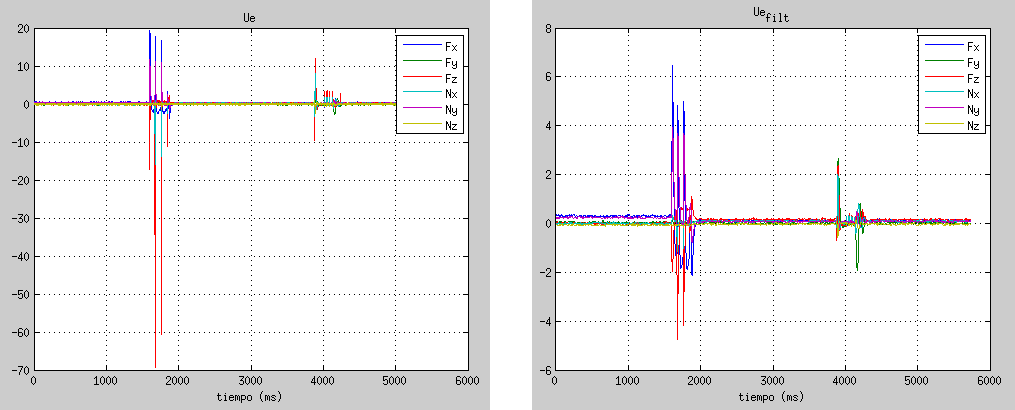
\includegraphics[scale=0.4]{Figuras/cmsf-WRSAlento}
\caption[Ensayo 12. Fuerza estimada con movimiento y sin fuerza]{Ensayo 12. Fuerza estimada con movimiento y sin fuerza: se efectúa un movimiento alrededor de la articulación \acrshort{wr} y \acrshort{sa} con controlador a menor velocidad. A la izquierda: fuerza externa estimada por el algoritmo. A la derecha: fuerza estimada filtrada.}
\label{fig:cmsf-WRSAlento}
\end{figure}

Tanto en el ensayo 11, como en el 12, se aprecia que la reducción de la velocidad del manipulador no supone una diferencia significativa en cuanto a los resultados obtenidos se refiere, por lo que la pérdida en operabilidad que supone la limitación de la velocidad máxima no es compensada por una mejora en las estimaciones, por lo que esta propuesta es desestimada. \par 

\end{itemize}

\subsubsection{Con movimiento y con fuerza externa}

Por último se considerará el caso más completo en el que se aúna la aplicación de una fuerza externa y un movimiento del manipulador. \par 

En vistas a los resultados obtenidos en el anterior apartado en los que la compensación dinámica no es efectuada correctamente sin aplicación alguna de fuerza externa, no cabe esperar un resultado más satisfactorio en este caso más completo. Igualmente a continuación se muestran los ensayos efectuados bajo estas condiciones. \par 

\begin{itemize}
\item \textbf{\emph{Ensayo 13}}: Se efectúa un giro de 1 radián alrededor del primer grado de libertad: la articulación \acrshort{sa}, mientras se ejerce una fuerza de -20 N en dirección del eje $z$ (figura \ref{fig:cmcf-SA-Fz}). \par 

\begin{figure}[h!]
\centering
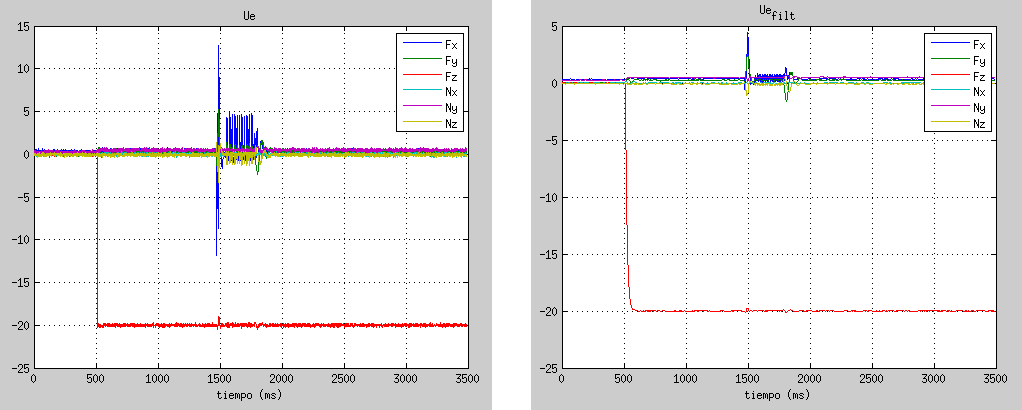
\includegraphics[scale=0.4]{Figuras/cmcf-SA-Fz}
\caption[Ensayo 13. Fuerza estimada con movimiento y con fuerza]{Ensayo 13. Fuerza estimada con movimiento y con fuerza: se efectúa un movimiento alrededor de la articulación \acrshort{sa} ejerciéndose una fuerza de -20 N a lo largo del eje $z$ con controlador. A la izquierda: fuerza externa estimada por el algoritmo. A la derecha: fuerza estimada filtrada.}
\label{fig:cmcf-SA-Fz}
\end{figure}

Se pretende simular mediante este ensayo el movimiento del manipulador mientras mantiene cierto objeto sujeto con el elemento terminal, sometido, por tanto, a su peso. El movimiento es efectuado mediante instrucciones del controlador, como puede apreciarse en la gráfica \ref{fig:cmcf-SA-Fz}, en las oscilaciones típicas del control de posición del controlador del \emph{grips} en \emph{gazebo}. \par 

Puede apreciarse el instante en el que se inicia el movimiento debido a las irregulares aceleraciones producidas por el controlador. La fuerza externa aplicada aparece, no obstante, perfectamente reflejada en la estimación. \par 

\item \textbf{\emph{Ensayo 14}}: Se efectúa un giro de 1 radián alrededor del primer grado de libertad: la articulación \acrshort{sa}, mientras se ejerce un momento de 7 N y -7 N en dirección del eje $z$ (figura \ref{fig:cmcf-SA-Nz}). \par 

\begin{figure}[h!]
\centering
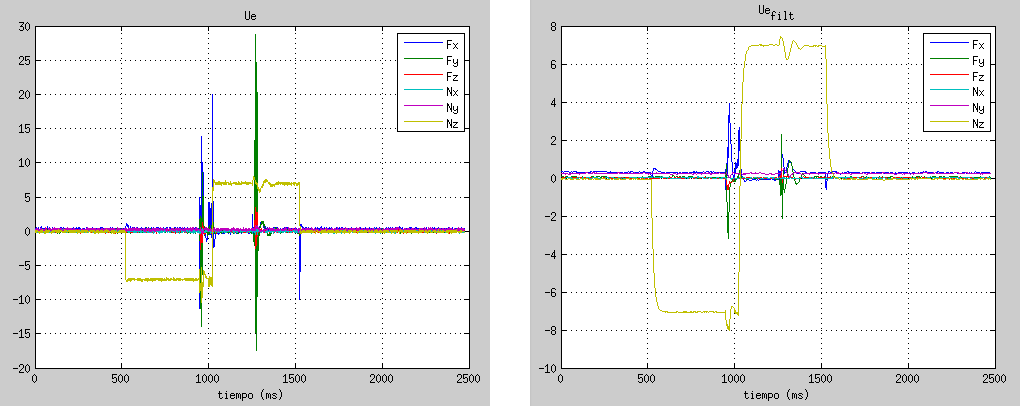
\includegraphics[scale=0.4]{Figuras/cmcf-SA-Nz}
\caption[Ensayo 14. Fuerza estimada con movimiento y con fuerza]{Ensayo 14. Fuerza estimada con movimiento y con fuerza: se efectúa un movimiento alrededor de la articulación \acrshort{sa} y \acrshort{wr} ejerciéndose un momento de 7 Nm y -7 Nm alrededor del eje $z$ con controlador. A la izquierda: fuerza externa estimada por el algoritmo. A la derecha: fuerza estimada filtrada.}
\label{fig:cmcf-SA-Nz}
\end{figure}

Puede observarse en este ensayo que el resultado de la estimación obtenida responde a una combinación de comportamientos de los ensayos 7 y 8. \par  

\item \textbf{\emph{Ensayo 15}}: Se efectúa un giro de 1 radián alrededor del primer grado de libertad: la articulación \acrshort{sa}, sin controlador, mientras se ejerce una fuerza de -20 N en dirección del eje $z$ (figura \ref{fig:cmcf-SAsc-Fz}). \par 

\begin{figure}[h!]
\centering
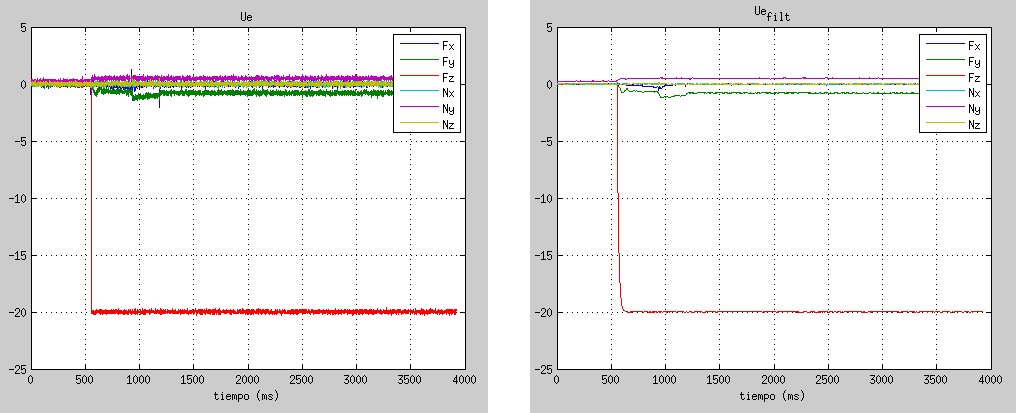
\includegraphics[scale=0.4]{Figuras/cmcf-SAsc-Fz}
\caption[Ensayo 15. Fuerza estimada con movimiento y con fuerza]{Ensayo 15. Fuerza estimada con movimiento y con fuerza: se efectúa un movimiento alrededor de la articulación \acrshort{sa} ejerciéndose una fuerza de -20 N a lo largo del eje $z$ sin controlador. A la izquierda: fuerza externa estimada por el algoritmo. A la derecha: fuerza estimada filtrada.}
\label{fig:cmcf-SAsc-Fz}
\end{figure} 

\item \textbf{\emph{Ensayo 16}}: Se efectúa un giro de 1 radián alrededor del primer grado de libertad: la articulación \acrshort{sa}, sin controlador, mientras se ejerce un momento de 7 N y -7 N en dirección del eje $z$ (figura \ref{fig:cmcf-SA-Nz}). \par 

\begin{figure}[h!]
\centering
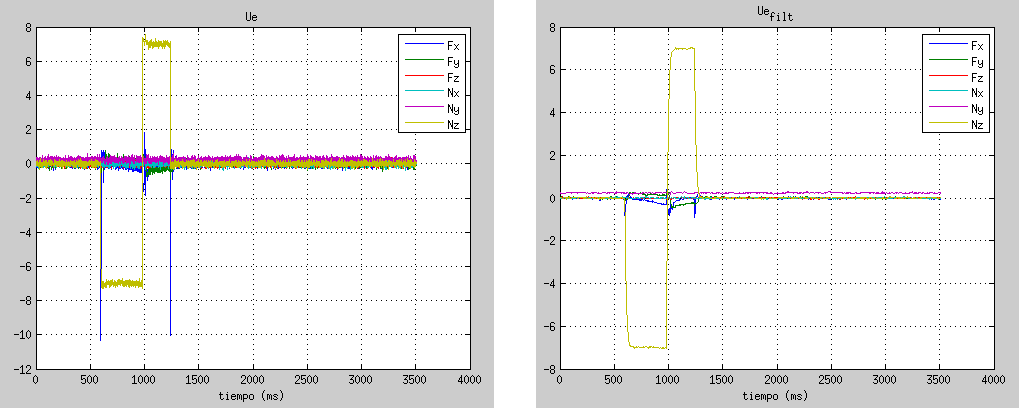
\includegraphics[scale=0.4]{Figuras/cmcf-SAsc-Nz}
\caption[Ensayo 16. Fuerza estimada con movimiento y con fuerza]{Ensayo 16. Fuerza estimada con movimiento y con fuerza: se efectúa un movimiento alrededor de la articulación \acrshort{sa} y \acrshort{wr} ejerciéndose un momento de 7 Nm y -7 Nm alrededor del eje $z$ sin controlador. A la izquierda: fuerza externa estimada por el algoritmo. A la derecha: fuerza estimada filtrada.}
\label{fig:cmcf-SAsc-Nz}
\end{figure} 

\end{itemize}

Puede apreciarse en estos dos últimos ensayos una notoria mejoría de las estimaciones debido a que el movimiento producido en estos casos es más uniforme y con aceleraciones y deceleraciones de menor magnitud que las originadas por el sistema de control del manipulador. Es preciso, por tanto, verificar y comprobar, al realizar una implantación en un sistema real del algoritmo presentado en el presente texto, si el sistema de control presenta comportamientos como los experimentados durante los ensayos mostrados. \par 

En general, puede concluirse que el estimador es extremadamente sensible, siendo su respuesta instantánea, sin retraso apreciable entre la aplicación de la fuerza y su detección. \par 

Debido al ruido existente en la estimación es imprescindible someter la señal a un proceso de filtrado, de manera que elimine el ruido sin comprometer la detección de esfuerzos por parte del algoritmo. \par 

En el próximo capítulo se desarrollarán en mayor medida las conclusiones extraídas de los experimentos efectuados. \par 

\section{Consideraciones éticas y sociales referentes al trabajo}

Debido al carácter de investigación que presenta el presente trabajo, difícilmente pueden destacarse aspectos éticos o sociales sin tener en cuenta la aplicación o uso que pueda darse a los resultados obtenidos con el mismo. De esta manera, las consideraciones éticas y sociales mencionadas, debido al objetivo de ser empleado el trabajo realizado en sistemas teleoperados, harán referencia a los aspectos derivados de la telerrobótica. \par 

Recuérdese que la teleoperación surge por la necesidad de extender la acción humana en ambientes peligrosos o dañinos para la salud. En esta línea debe proseguir el desarrollo de la robótica. \par 

La inclusión de la telerrobótica en distintos ámbitos de la vida, ya puedan ser sanitarios, como el uso de robótica en cirugías, que permiten un control más preciso de las operaciones a realizar, o en reparaciones de dispositivos en el espacio o en centrales nucleares, saca a la luz el gran potencial existente para la humanidad del uso de esta tecnología con el fin de extender las capacidades humanas. \par 

Es preciso resaltar, por último, el uso del sistema empleado en el presente trabajo, formado por el manipulador robótico de \emph{Kraft Telerobotics, Inc.}, para la reparación de líneas de alta tensión. Este ejemplo de aplicación muestra a su vez, el tipo de aplicaciones en las que se puede dar uso de los trabajos realizados. \par 